\documentclass[a4paper, 11pt]{article}

%%% Zeichenkodierung, Rechtschreibung und Umlaute
\usepackage[utf8]{inputenc}
\usepackage[ngerman]{babel}
\usepackage[T1]{fontenc}

%%% Mathematische Symbole, Gleichungen
\usepackage[fleqn]{amsmath}
\usepackage{amsfonts}
\usepackage{amssymb}
\usepackage{amsthm}
\usepackage{mathtools}
\usepackage{bm}
%\usepackage{colonequals} % Zusätzliche Relationssymbole

%%% Tabellen
\usepackage{tabularx}
\usepackage{array}
\usepackage{multicol}

%%% Seitenformat und -ränder
%%% -Alternative 1-
\usepackage{geometry}
\geometry{a4paper, top=25mm, bottom=20mm, left=20mm, right=20mm}
%%% -Alternative 2-
%\usepackage[headheight=110pt]{geometry}
%\geometry{a4paper,left=30mm,right=30mm, top=35mm, bottom=30mm}

%%% Seitenstile (Kopf- und Fußzeile)
\usepackage{fancyhdr}
\pagestyle{fancy}

%%% Sonstiges
\usepackage{caption} % Untertitel von Grafiken/Tabellen manipulieren
\usepackage{enumerate} % Aufzählungszeichen ändern
\usepackage{graphicx} % Standarderweiterung für Bilddateien
\usepackage{hyperref} % Hyperlinks
\usepackage{lastpage} % Berechnung der Seitenzahl
%\usepackage{polynom} % Polynomdivision
\usepackage{setspace} % Zeilenabstand
%\usepackage{textgreek} % griechische Symbole
\usepackage{tikz} % Umfassendes Tool, um Grafiken zu erstellen
\usepackage{verbatim} % Schreibmaschinen-Stil (für Code-Ausschnitte)
\usepackage{float}

%%% Eingaben (z.B. für das Deckblatt)
\newcommand{\moduleabrv}{EDS}
\newcommand{\module}{Embedded System Design Protokoll}
\newcommand{\semester}{Beuth Hochschule - Sommersemester 2018}
\newcommand{\finishingdate}{15.09.2018}
\newcommand{\titletextabrv}{       A/V Streaming}
\newcommand{\titletext}{Audio Video Streaming}

%%%-- Für das Deckblatt --
\title{
	~\\[4cm]
	\textbf{
		\module\\[0.25cm]
		\normalsize \semester \\[1.5cm]
		\Huge\titletext\\
	}
}

\author{
  \vspace{3.5cm}\\
  \begin{tabular}{l}
    \textbf{Gruppe 15:}\\\hline
    Omid Rahimian Mashhadi \\
    Torsten Michael Schenk Mat.Nr.: 838995\\
  \end{tabular}
}

\date{
	\vfill
	Abgabedatum: \finishingdate\\
	\vspace{5mm}
	Seitenanzahl: \pageref{LastPage}
}

%%% -- Kopf- und Fußzeile --
%%% Kopfzeile linker Bereich
\lhead[\leftmark]{\textbf{\moduleabrv}}
%%% Kopfzeile mittlerer Bereich
\rhead[\rightmark]{\rightmark{\titletextabrv}}
%%% Kopfzeile linker Bereich
%%\rhead{\textbf{zum \finishingdate}}
%%% Fußzeile
\cfoot{\thepage  \ / \pageref{LastPage}}

%%% Serifenfreie Fonts benutzen
%\renewcommand{\familydefault}{\sfdefault}

%%% Font
\usepackage{charter}

%%% Tiefe der Einrückung nach Absätzen
\setlength{\parindent}{0pt}

%%% Evtl. Änderungen des Typs einer Aufzählungsebene (z.B. zur Anpassung an das Aufgabenblatt)
%\renewcommand{\labelenumi}{\alph{enumi})}
%\renewcommand{\labelenumii}{(\roman{enumii})}
%\renewcommand{\labelenumiii}{\arabic{enumiii}.}
%\renewcommand{\labelenumii}{\textbf{-}}

\begin{document}

%%% Deckblatt
\maketitle
\thispagestyle{empty} % Keine Seitenzahl hier

\newpage
%\renewcommand\contentsname{Inhalt}
%\tableofcontents
    {\pagestyle{plain}
    \tableofcontents
    \cleardoublepage
    }

%\newpage
%%% Seitenzahl zurücksetzen
%\clearpage
%\setcounter{page}{1}

%%% Zeilenabstand
%\singlespacing
\onehalfspacing
%\doublespacing

%%%-- Eigentlicher Inhalt --
\section{Vorwort}
Für den Support und Bereitstellung von Hardware bedanken wir uns herzlich bei Herrn Krinke von der pi4\_robotics GmbH Berlin und für die beratende Funktion danken wir den Dozenten und Professoren der Beuth Hochschule Prof. Löwis, Dr. Flemming und Prof. Görlich.\\
Bei der Recherche zur Bearbeitung des Projektes wurden viele englische Webseiten zu rate gezogen und auch die man-pages der meisten Programme sind in Englisch verfasst. Generell kann man sagen, dass englische Fachbegriffe sich im Bereich Software etabliert haben, so dass eine Übersetzung eher verwirren als helfen würde. Daher haben wir uns entschieden, die \textbf{englischen} Bezeichner und Beschreibungen von Flags und Optionen beizubehalten.\\
Um Codeabschnitte besser von Beschreibungen unterscheiden zu können, wurde eine eigene Schriftart verwendet:
\begin{verbatim}
  Kommandozeilen Eingaben und Codesnippets werden wie HIER dargestellt.
\end{verbatim}

\section{Projektbeschreibung}
Das erklärte Ziel der pi4\_robotics GmbH Berlin ist es humanoide Roboter weiter zu entwickeln. 
Diese können bereits in unterschiedlichen Branchen eingesetzt werden. Im Werbeblatt 
des Workerbot4 (siehe Anhang, Kapitel 13) werden die Basisfähigkeiten des Jolandi Workerbot beschrieben.  \\
Bisher ist das Anlernen neuer Tätigkeiten und die Bedienung nur über eine PC-Schnittstelle möglich, doch das soll sich ändern. Es ist geplant Spracherkennung und visuelle Wahrnehmung 
zu integrieren. Um mit dem Roboter wie mit einem Menschen kommunizieren zu können. Auch soll 
ein Avatar Modus implementiert werden, bei dem der User in die Rolle des Roboters schlüpft 
und per Teleoperation den Roboter bewegt, hört was der Roboter hört und mit den Augen des Roboters sieht. \\
\begin{minipage}{\textwidth}
    \begin{center}
        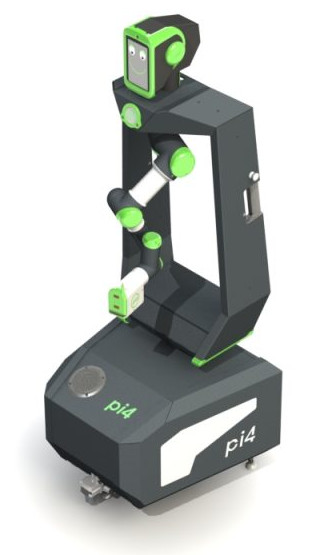
\includegraphics[scale=0.5]{img/jolandi.jpg} 
    \end{center}
\end{minipage}
\begin{center}
Jolandi Workerbot der Firma pi4\_robotics GmbH
\end{center}
 
\begin{minipage}{\textwidth}
    \begin{center}        
        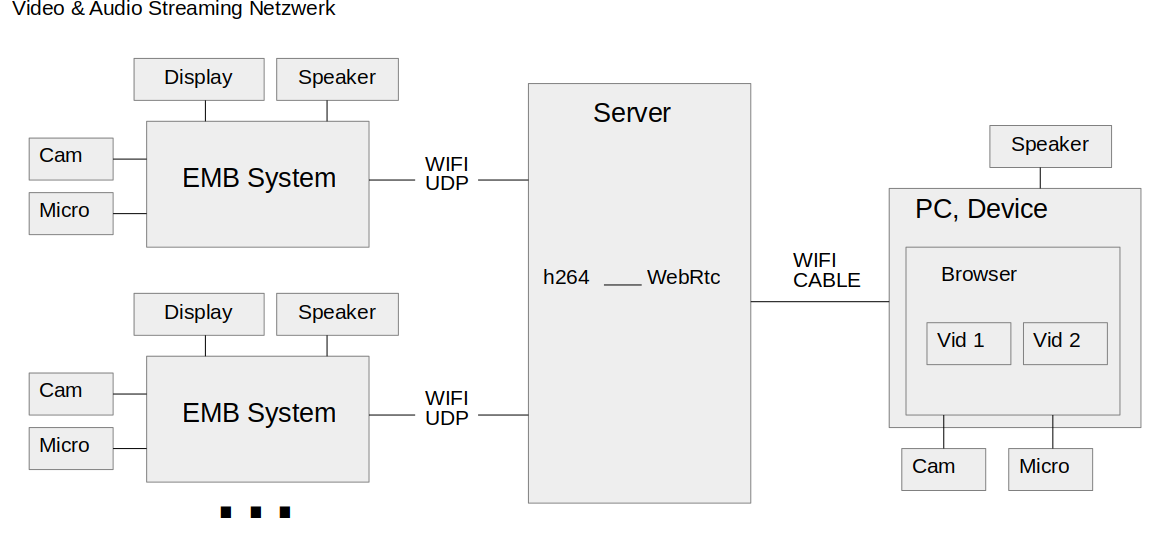
\includegraphics[scale=0.4]{img/schemaproj.png} 
    \end{center}
\end{minipage}
\begin{center}
Schemaplan der Komponenten
\end{center}
Für den Einsatz als Sicherheitspersonal ist weiterhin geplant, die Stimme des Bedieners aus dem Roboter Lautsprecher ertönen zu lassen und sein Gesicht auf dem Kopfdisplay anzuzeigen. 
Der Kunde soll das Gefühl haben, dass der Roboter der Avatar des Bedieners ist.\\
Für die Laborübungen 'Entwurf eingebetteter Systeme' und 'Netzwerk-Programmierung' wurde 
bidirektionale Ton und Video Übertragung ausgewählt. Dabei galt es Audio und Video \textbf{mehrerer} Roboter auf eine Webseite zu streamen und eine Webcam inklusive Ton des PC auf alle verbundenen Roboter zurück zu streamen.\\

Der Schemaplan zeigt den grundlegenden Aufbau des Komplettsystems. Auf der linken Seite sind 'n' integrierte eingebettete Systeme gezeigt, wie sie in pi4\_robotics GmbH Robotern verbaut sind. Pro Roboterkopf ist ein Raspberry PI mit Touch-Display vorhanden. Für das Projekt wurde jeweils eine Webcam für Ton und Video angeschlossen. Die Tonwiedergabe erfolgt über einen USB Lautsprecher. Die Anzeige des empfangenen Videostreams soll \textbf{ohne} Webbrowser erfolgen.\\
Auf der rechten Seite des Plans ist der Bediener PC dargestellt. Auch hier liefert eine Webcam Ton und Video. Der empfangene Audiostream wird über die PC Lautsprecher ausgegeben.\\
Für den Bediener soll ein \textbf{Web-Template} erstellt werden. Dort kann dieser auswählen, welcher Videostream angezeigt werden soll. Der Zeitversatz bei der Übertragung soll sehr gering sein 
(<0.2sek), damit der User möglichst schnell reagieren kann. Bildübertragung zum eingebetteten System darf einen leichten Zeitversatz haben, da dort nur das Gesicht des Bedieners angezeigt wird, aber keine weiteren Handlungen davon abhängen.\\
Das gesamte Streaming soll über das Internet erfolgen. Dabei ist der Datentransfer auch aus 
fremden WLAN Netzen heraus zu realisieren. Fremd im Sinne, dass die dazwischen liegenden Router und Ports nicht konfiguriert werden können. Die IP Adressen der Roboter sind damit quasi unbekannt, d.h. dynamisch wechselnd oder/und nicht vom Internet aus sichtbar, d.h. es ist nicht möglich direkt vom Sender zum Empfänger zu streamen.\\
Eine weitere Anforderung war den Datentransport möglichst Effizient zu gestalten. Für den Upload ins Internet sollte ein Transportprotokoll mit geringem Overhead gewählt werden und für das Streaming auf die Webseite ein natives Format, welches von aktuellen Browsern unterstützt wird. Die Visualisierung sollte in Html5 \& Javascript ohne Browser-Plugins, Flash o.ä. erfolgen. Für die Realisierung musste also eine Möglichkeit gefunden werden, das Upload Format zu konvertieren und die Webseite mit einem Audio- und Videostream zu versorgen. Eine Streaminglösung über das Web erfordert drei Basiskomponenten um die Aufgabe zu erfüllen. Einen Streaming Server, einen Sender und einen Empfänger.

\textbf{Streaming-Server:} 
Ist die Hauptkomponente, die Audio- und Videoinhalte von den Sendern an die Empfänger weiterleitet. Gleichzeitig kann auch die Konvertierung von einem Format oder Codec in ein anderes erfolgen.

\textbf{Sender:} Eine Quelle, die einen Audio- und Videostream zum Server schickt. 

\textbf{Empfänger:} Ein Empfänger, der sich mit dem Stream vom Server verbindet und diesen abspielt oder speichert.
\section{Realisation}
Schon bei Projektstart wurde klar, dass es sich um sehr umfangreiche Anforderungen handelt. Es galt nicht nur eine Streaming Lösung zu implementieren, sondern es mussten auch alle Hardwarekomponenten getestet und angesteuert werden. Für die Bedienerseite musste eine funktionale Webseite einschließlich Webserver erstellt werden und ein Streaming-Server für die Konvertierung und Vernetzung der Sender und Empfänger musste konfiguriert werden. Viele \textbf{wichtige} bisher nicht genannte Anforderungen, z.B. Cybersicherheit, Authentifizierung wurden weitestgehend außer acht gelassen. Sie sind natürlich für eine endgültige industrielle Anwendung unerlässlich.\\

Das Projekt wurde in Teil-Aufgaben realisiert:
\begin{itemize}
\item Inbetriebnahme aller Hardwarekomponenten

\item Direktes Streamen von Audio und Video von embedded System an PC
\item Aufsetzen eines Webservers im lokalen Netzwerk, lokales hosting der Webseite
\item Aufsetzen eines Streaming-Servers im lokalen Netzwerk
\item Direktes Streamen von Audio und Video von embedded System an Streaming-Server
\item Anzeige des konvertierten Outputs des Streaming-Servers auf der Webseite

\item Streamen der PC Webcam an lokalen Streaming-Server
\item Zurück-Streamen vom Streaming-Server an embedded Hardware und Visualisierung

\item Hochladen der Webseite auf eine Online-Webspace
\item Aufsetzen eines Online-Streaming-Servers
\end{itemize}

\subsection{Hardware Inbetriebnahme der Komponenten}
Beschreibung...\\

\subsection{Streamen vom embedded System: Streaming-Server \& Webserver}
Beschreibung...\\

\textbf{Direktes StreamEN von Audio und Video von embedded System an PC}\\
blah blah blah\\

\textbf{Aufsetzen eines Webservers im lokalen Netzwerk, lokales hosting der Webseite}\\
blah blah blah\\

\textbf{Aufsetzen eine Streaming-Servers im lokalen Netzwerk}\\
blah blah blah\\

\textbf{Direktes Streaming von Audio und Video von embedded System an Streaming-Server}\\
blah blah blah\\

\subsection{Webseite zur Anzeige der Videostreams}
Beschreibung...\\

\textbf{Anzeige des konvertierten Outputs des Streaming-Servers auf der Webseite}\\
blah blah blah\\

\subsection{Streamen von PC: Streaming-Server \& Anzeige auf embedded Sytem}
Beschreibung...\\

\textbf{Streamen der PC Webcam an lokalen Streaming-Server}\\
blah blah blah\\

\textbf{Zurück-Streamen vom Streaming-Server an embedded Hardware und Visualisierung}\\
blah blah blah\\

\subsection{Online Setup}
Beschreibung...\\

\textbf{Hochladen der Webseite auf eine Online-Wespace}\\

Hochladen der Webseite via Filezilla...\\

\textbf{Aufsetzen eines Online-Streaming-Servers}\\
blah blah blah\\

\textbf{Webserver Verbindungstest}\\
Im oberen Bereich ist der gstreamer Befehl mit dem Audio udpsink host...5000 und Video udpsink...5001. Wireshark detektiert ankommende Pakete im Webserver (ip 85.214.211.169) vom raspberry pi (ip 77.14.37.230) an den UDP Ports 5000 (Audio Paketgröße 451) und UDP 5001 (Video Paketgröße 894).\\

\begin{minipage}{\textwidth}
    \begin{center}
        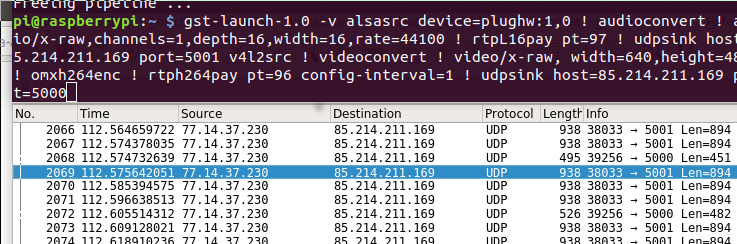
\includegraphics[scale=0.85]{img/wireshark.png} 
    \end{center}
\end{minipage}

\newpage
\section{Software}

%%%%%%%%%%%%%%%%%%%%%%%%%%%%%%%%%%%%%%%%%%%%%%%%%%%%%%%%%%%%%%%%%%%%%%%%%%
\subsection{Raspberry Touchscreen Anzeige per Software Drehen}
Wenn das Raspberry 7\grqq{} Display ins Gehäuse eingebaut wird ist die 
Visualisierung des Desktops 180 Grad verdreht. Es müssen Bildschirmanzeige 
und Toucherkennung gedreht werden. Softwaretechnisch sind dies zwei verschiedene 
Dinge.\\

\textbf{RASPIAN OP}\\
Display \& Touchscreen können mit einem Befehl rotiert werden, 
bitte in /boot/config.txt eintragen:
\begin{verbatim}lcd_rotate=2\end{verbatim}

\textbf{Andere OP}\\
Hier wird mittels des lcd\_display Befehls nur der Touchbildschrim 
gedreht. Es kann xrandr verwendet werden um zusätzlich die visuelle Darstellung zu 
um 180 Grad zu drehen. Display Infos \& drehen:
\begin{verbatim}
xrandr -q
xrandr --output HDMI-1 --rotate inverted
\end{verbatim}


%%%%%%%%%%%%%%%%%%%%%%%%%%%%%%%%%%%%%%%%%%%%%%%%%%%%%%%%%%%%%%%%%%%%%%%%%
\subsection{ffmpeg, ffserver, ffplay}

\textbf{Linux / Raspian ffmpeg mit alsa} %and pi\_jessie\_motion}
   
REWORK in GERMAN:\\
No, unfortunately not. You must recompile ffmpeg to add enable additional libraries. Below is the script I build to compile ffmpeg with alsa, fdk-aac, and libx264 support. It will install ffmpeg in your home folder inside a "ffmpeg" folder, so you'll need to call it specifically from there unless you add it to your path. I recommend uninstalling your current ffmpeg before using my script.

Btw, I am able to stream directly to YouTube now without any issues. I use an external USB sound card and the PiCam v2 and stream a 1920x1080@25fps video stream with a 192kbps stereo audio stream mixed in. It works great!\\

Wichtige Info, ffserver wurde beim Upgrade auf ffmpeg Version 4.0 gelöscht. Letzte Version mit ffserver ist 3.4. Daher git checkout 3.4!

Installation von FFmpeg aus Source-Code: 
\begin{verbatim}
#!/bin/bash
# My first script
# 
# to install ffserver, you have to check out the 3.5 of 3.4 version of ffmepg git repo
# to be able to compile ffmpeg with x264, you also have to choose an old version from git repo
# tested was the version, before x264_bit_depth was removed (needed for ffmpeg 3.4, 3.5)
# x264 hash key checkout: 7839a9e1f03b49e3e0cbfcb3091093af7c6d54ee
#
wget http://downloads.xiph.org/releases/vorbis/libvorbis-1.3.3.tar.gz
tar -xf libvorbis-1.3.3.tar.gz
cd libvorbis-1.3.3/
./configure --host=arm-unknown-linux-gnueabi --enable-static
make
sudo make install
cd ..
# libogg
wget http://downloads.xiph.org/releases/ogg/libogg-1.3.1.tar.gz
tar -xf libogg-1.3.1.tar.gz
cd libogg-1.3.1/
./configure --host=arm-unknown-linux-gnueabi --enable-static
make
sudo make install
cd ..
# libtheora
wget http://downloads.xiph.org/releases/theora/libtheora-1.1.1.tar.bz2
tar -xf libtheora-1.1.1.tar.bz2
cd libtheora-1.1.1/
./configure --host=arm-unknown-linux-gnueabi --enable-static
make
sudo make install
cd ..
git clone http://git.videolan.org/git/x264.git
cd x264
./configure --host=arm-unknown-linux-gnueabi --enable-static --disable-opencl
echo "Compiling x264"
make
sudo make install
cd ..
# extra alsa
wget ftp://ftp.alsa-project.org/pub/lib/alsa-lib-1.1.1.tar.bz2
tar xjf alsa-lib-1.1.1.tar.bz2
cd alsa-lib-1.1.1/
./configure --host=arm-unknown-linux-gnueabi --enable-static
make -j4
sudo make install
cd ..
# libvpx
git clone https://chromium.googlesource.com/webm/libvpx
cd libvpx
./configure --enable-static
make -j4
sudo make install
cd ..
# libsdl
wget http://www.libsdl.org/release/SDL-1.2.15.tar.gz
tar xzvf SDL-1.2.15.tar.gz
cd SDL-1.2.15
./configure --host=arm-unknown-linux-gnueabi --enable-static
make -j4
sudo make install
cd ..
git clone https://github.com/FFmpeg/FFmpeg.git
cd ffmpeg
./configure --arch=armel --target-os=linux --enable-gpl --enable-libx264 --enable-nonfree --enable-libtheora --enable-libvorbis --enable-libvpx
make
sudo make install
\end{verbatim}	

Als erste Tests kann ffmpeg dazu verwendet werden Videos mit oder ohne Audio zu speichern.\\
Dabei traten beim .ogg Format ungewöhnliche Speed-Ups oder Sprünge statt. Mp4 ist von 
ausgezeichneter Qualität. Tests ohne Audio:
\begin{verbatim}
ffmpeg -f v4l2 -r 25 -s 640x480 -i /dev/video0 out.avi
ffmpeg -f v4l2 -r 25 -s 640x480 -i /dev/video0 out.mp4
ffmpeg -f v4l2 -r 25 -s 640x480 -i /dev/video0 out.ogg
\end{verbatim}

Test mit Audio:
\begin{verbatim}
arecord -D plughw:1,0 -f cd test.wav
mplayer test.wav
\end{verbatim}


Danach kann über den ffserver auf eine Webpage gestreamt werden:\\
ffserver.config
\begin{verbatim}
HTTPPort 9090
HTTPBindAddress 0.0.0.0
MaxHTTPConnections 2000
MaxClients 1000
MaxBandwidth 100000
#NoDaemon

<Feed feed1.ffm>
        File /tmp/feed1.ffm
        FileMaxSize 200K
        ACL allow 127.0.0.1
</Feed>

<Stream test.ogg>
        Format ogg
        Feed feed1.ffm

        VideoCodec libtheora
        VideoFrameRate 24
        VideoBitRate 512
        VideoSize 320x240
        VideoQMin 1
        VideoQMax 31
        VideoGopSize 12
        PreRoll 0
        AVOptionVideo flags +global_header
        Noaudio
</Stream>

<Stream stat.html>
        Format status
        # Only allow local people to get the status
        ACL allow localhost
        ACL allow 192.168.0.0 192.168.255.255
</Stream>                         
\end{verbatim}

Start ffserver und ffmpeg:
\begin{verbatim}
ffserver -f ffserver.config
ffmpeg -f v4l2 -i /dev/video0 -vcodec libtheora http://localhost:9090/feed1.ffm
\end{verbatim}
	
% Aufzeichnen von wav mit ffmpeg:
% \begin{verbatim}./ffmpeg -f alsa -i hw:1 alsaout.wav \end{verbatim}
% abspielen:
% \begin{verbatim}aplay alsaout.wav \end{verbatim}
% Aufzeichnen von webm mit ffmpeg:
% \begin{verbatim}
% ./ffmpeg -f alsa -i hw:1 -strict experimental alsaout.webm  
% ACHTUNG: bei ffmpeg dürfen keine Anführungszeichen um plughw gesetzt werden!
% webcam: ./ffmpeg -f alsa -i plughw:CARD=C920,DEV=0 -strict experimental alsaout.webm
%
% \end{verbatim}
% abspielen:
% \begin{verbatim}
%
% \end{verbatim}


%%%%%%%%%%%%%%%%%%%%%%%%%%%%%%%%%%%%%%%%%%%%%%%%%%%%%%%%%%%%%%%%%%%%%%%%%%%
\subsection{Motion Installation \& Test}

Motion ist ein Programm, das in der Lage ist zu erkennen, wenn ein signifikanter Teil des Kamerabildes sich verändert. Es kann also 
Bewegung erkennen und einen Warnton übertragen. Kamera streaming 
Service welches verwendet werden kann, um den Videostream 
einer Webcam an eine IP Adresse zu leiten. Motion kann mit 
vielen Geräten verwendet werden. Unterstützt werden:
\begin{itemize}
\item V4L2 Webcams (closed source)
\item Video Frame Grabber
\item Network Kameras via HTTP, RTSP, RTMP
\item PI Kameramodul
\item Webcam
\end{itemize}

Video Stream zur IP Adresse des Devices (Raspi) im es im lokalen 
Netzwerk um Browser anzuzeigen....TODO

OP: Raspian\\
Setup: Streaming server motion\\

Anleitung nach Tutorial mit Anpassungen:\\
https://pimylifeup.com/raspberry-pi-webcam-server/\\

\textbf{Jessie and Strech are two debian major release}\\
Debian 9 (stretch) — current stable release\\
Debian 8 (jessie) — obsolete stable release\\

\textbf{Raspian pi\_strech\_motion}

\begin{enumerate}
	\item install:\\
	sudo apt-get install libmariadbclient18 libpq5 libavcodec57  libavformat57 libavutil55 libswscale4\\
	einige Pakete sind outdated und müssen durch aktuelle ersetzt werden:\\
	sudo apt install libx264-148\\
	libavcodec57\\
	libavformat57\\
	libmariadbclient-dev-compat\\
	default-libmysqlclient-dev\\
	libswscale

	\item download motion stretch deb\\
	sudo wget https://github.com/Motion-Project/motion/releases/download/release-4.0.1/pi\\
	\_stretch\_motion\_4.0.1-1\_armhf.deb
	
	sudo dpkg -i pi\_stretch\_motion\_4.0.1-1\_armhf.deb\\

	Configuring Motion:\\
	sudo vim /etc/motion/motion.conf\\
	daemon on\\
	stream\_localhost off\\
	if problems with freezing if motion occures\\
	output\_pictures off\\
	ffmpeg\_output\_movies off\\
	optional\\
	stream\_maxrate 100\\
	framerate 100\\
	width 640\\
	height 480

	\item setup daemon\\
	sudo vim /etc/default/motion\\
	start\_motion\_daemon=yes
\end{enumerate}

start stop motion and streaming by:\\
sudo service motion start\\
sudo service motion stop\\

check browser in local network, xxx ip adress of raspi (ip addr show):\\
192.168.1.xxx:8081

How to test if video and avi works at all:\\
Test raspi video codex and sound from avi video\\
omxplayer -p -o local dolbycanyon.avi\\
-o local = headphone jack

%%%%%%%%%%%%%%%%%%%%%%%%%%%%%%%%%%%%%%%%%%%%%%%%%%%%%%%%%%%%%%%%%%%%%%%%%%
\subsection{gstreamer}

Wenn Fehler beim Compilieren eines gstream Testprogramms auftreten, z.B.
\begin{verbatim}
Package gstreamer-1.0 was not found in the pkg-config search path.
Perhaps you should add the directory containing `gstreamer-1.0.pc'
to the PKG_CONFIG_PATH environment variable
No package 'gstreamer-1.0' found
playback-tutorial-6.c:1:10: fatal error: gst/gst.h: No such file or directory
\end{verbatim}

gstreamer-1.0 ist der folgenden lib enthalten:\\
sudo apt install libgstreamer1.0-dev\\

\textbf{Beispiel Programme gstreamer kompilieren}
gcc playback-tutorial-6.c -o playback-tutorial-6 `pkg-config --cflags --libs gstreamer-1.0`

%%%%%%%%%%%%%%%%%%%%%%%%%%%%%%%%%%%%%%%%%%%%%%%%%%%%%%%%%%%%%%%%%%%%%%%%%%


\newpage
\section{Hardware}

%%%%%%%%%%%%%%%%%%%%%%%%%%%%%%%%%%%%%%%%%%%%%%%%%%%%%%%%%%%%%%%%%%%%%%%%%%%%%%%%%%%%%%%%%%%%%%%%%%%%
\subsection{Raspberry Pi 3B+}
\textbf{Login via ssh}\\
Passwort und Benutzername können bereits bei der OP-Installation gesetzt werden.\\
IP-Adresse kann über ip addr show abgefragt werden. Bei häufigen Verbindungen wird empfohlen 
eine statische IP-Adresse zu vergeben.\\
ssh pi@192.168.1.3\\
pwd: xxxxxxxxxx (pwd vom Provider)

%%%%%%%%%%%%%%%%%%%%%%%%%%%%%%%%%%%%%%%%%%%%%%%%%%%%%%%%%%%%%%%%%%%%%%%%%%%%%%%%%%%%%%%%%%%%%%%%%%%%
\subsection{Strato Web Server}
\textbf{Login via ssh}\\
ssh -X root@85.214.211.169\\
ssh -X root@85.214.211.169 -L 5901:localhost:5901\\
pwd: xxxxxxxxxx (pwd vom Provider)

\textbf{Remote Desktop}\\
tightvncserver: server\\
xtightvncviewer: viewer\\
sudo apt install tightvncserver xtightvncviewer\\
\# set xtightvnciewer pwd\\

\textbf{Full Login}\\
ssh -X root@85.214.211.169 -L 5901:localhost:5901\\
ssh Passwort eingeben\\
\# Start vncserver\\
vncserver :1\\
echo \grqq{}\$DISPLAY\grqq{}\\
\# in server ssh console\\
xtightvncviewer 127.0.0.1:1\\
vnc Passwort eingeben\\
\# X Fenster sollte sich öffnen\\

Dateien auf Server übertragen:
\begin{verbatim}
scp <source> <destination>
To copy a file from B to A while logged into B:
scp /path/to/file username@a:/path/to/destination
To copy a file from B to A while logged into A:
scp username@b:/path/to/file /path/to/destination
# upload: local -> remote
scp local_file user@remote_host:remote_file
scp /path/file.conf user@host:/path/file.conf
\end{verbatim}


%%%%%%%%%%%%%%%%%%%%%%%%%%%%%%%%%%%%%%%%%%%%%%%%%%%%%%%%%%%%%%%%%%%%%%%%%%%%%%%%%%%%%%%%%%%%%%%%%%%%%
\subsection{Audio Lautsprecher}
%Um Audio auf den Headphone Jack umzuleiten (default ist HDMI) zuerst pulseaudio deinstallieren.\\
%sudo apt remove pulseaudio\\

Die richtige Zuordnung setzen, sonst gibt es nur Sound vom 
abspielen von Audiodateien aber nicht im Browser. Bitte im 
Browser, z.B. mit YouTube. '1' steht für local audio jack über 
den den Lautsprecher angeschlossen ist:
\begin{verbatim}
amixer cset numid=3 1
amixer cset numid=2 1
oder
amixer -c 0 cset numid=3 1
\end{verbatim}

\textbf{Audio Tests}
\begin{verbatim}aplay /usr/share/scratch/Media/Sounds/Vocals/Singer1.wav\end{verbatim}
Facebook Video Call: OK (schlechter Sound)\\
Musikvidoes auf YoutTube: OK (guter Sound)\\

Kommandozeile, um alle Audiogeräte anzuzeigen:\\
pacmd list-sources

Listet alle *.ogg Audiodateien auf dem ubuntu Rechner auf:\\
pacmd list-samples\\
Lautsprechertest (abspielen):\\
mplayer /usr/share/sounds/ubuntu/stereo/button-pressed.ogg 

%%%%%%%%%%%%%%%%%%%%%%%%%%%%%%%%%%%%%%%%%%%%%%%%%%%%%%%%%%%%%%%%%%%%%%%%%%%%%%%%%%%%%%%%%%%%%%%%%%%%%%%
\subsection{Mikrofon der Webcam}
Anzeigen, ob Webcam erkannt wurde.\\
pacmd list-sources\\ 

Audio Stream aufnehmen:
\begin{verbatim}arecord -D plughw:1,0 -f cd test.wav\end{verbatim}
\#abspielen mit:
\begin{verbatim}aplay test.wav\end{verbatim}

Falls Hardwarekennung unbekannt, zeige alle Geräte:
\begin{verbatim}arecord -L\end{verbatim}
Interessant ist der letzte Eintrag plughw, diesen kann man direkt für
ffmpeg verwenden, z.B.:
\begin{verbatim}
webcam: ...plughw:CARD=C920,DEV=0 ...
usb-micro: arecord -D plughw:CARD=Device,DEV=0 -f cd test.wav
\end{verbatim}

Wenn beim Testen mit ffmpeg der Fehler: 
\textbf{Unknown input format: 'alsa'}\\ 
auftreten, muss ffmpeg aus den Quellen kompiliert werden, siehe 
Softwarekapitel oder\\ 
https://lb.raspberrypi.org/forums/viewtopic.php?t=205181


 
\newpage
\section{Definitionen \& Formate}
List aller Codex und Datei-Formate die während des Projektes zum Einsatz kamen.

%%%%%%%%%%%%%%%%%%%%%%%%%%%%%%%%%%%%%%%%%%%%%%%%%%%%%%%%%%%%%%%%%%%%%%%%%%%%%%%
\subsection{ogg}

\textbf{WIKIpedia - rewrite - Zusammenfassen}
Achtung, kann auch direkt auf einer Website dargestellt werden!\\

Ogg ist ein Container-Dateiformat für Multimedia-Dateien, kann also gleichzeitig Audio-, Video- sowie Textdaten enthalten. Ogg wurde mit dem Ziel konzipiert, eine freie und von Softwarepatenten unbeschränkte Alternative zu proprietären Formaten zu bieten, um Multimedia-Inhalte effizient zu speichern und zu streamen. Die Streamingfähigkeit ist dabei das entscheidende Designmerkmal: Alles, was in einem Ogg-Container verpackt ist, kann ohne zusätzliche Anpassungen gestreamt werden. Dies unterscheidet Ogg von Formaten, die entweder nur in bestimmten Ausprägungen streamingfähig sind (wie z. B. Matroska) oder überhaupt nicht live-streaming-fähig sind (wie z. B. MP4). Ogg-Streams können dabei gebündelt und verkettet werden, ohne dass dazu eine Anpassung des einzelnen Streams notwendig ist.[2]

Die Entwicklung des Container-Formats wird von der Xiph.Org Foundation geleitet, die auch für einige Codecs verantwortlich ist, welche die Inhalte in einem Ogg-Container komprimieren.

Der bekannteste Codec ist dabei der Audio-Codec Vorbis, welcher oft vereinfachend (oder auch irrtümlich) als Ogg bezeichnet wird, obwohl Ogg tatsächlich nur das Containerformat für die Vorbis-kodierten Inhalte ist. In jüngerer Vergangenheit (seit 2012) setzt sich auch das Vorbis-Nachfolgeformat Opus langsam durch, insbesondere auch im professionellen Broadcast-Umfeld in Hardware-Audio-Codecs. 


%%%%%%%%%%%%%%%%%%%%%%%%%%%%%%%%%%%%%%%%%%%%%%%%%%%%%%%%%%%%%%%%%%%%%%%%%%%%%%%
\subsection{h264}

Beschreibung des Projektes...

\begin{minipage}{\textwidth}
    \begin{center}
        Caption for image
        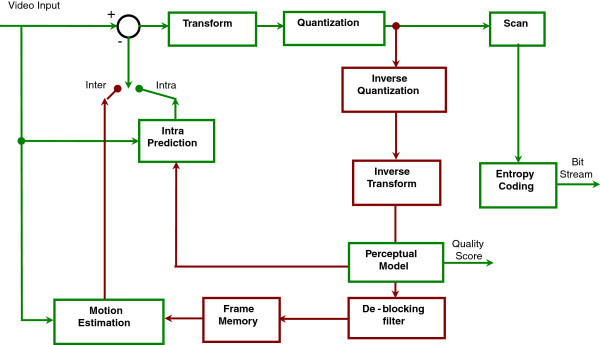
\includegraphics[scale=4.0]{img/h264.jpg} 
    \end{center}
\end{minipage}




%%%%%%%%%%%%%%%%%%%%%%%%%%%%%%%%%%%%%%%%%%%%%%%%%%%%%%%%%%%%%%%%%%%%%%%%%%%%%%%
\newpage
\section{Vergleich der Formate}

\subsection{RTMP versus WebRTC}
RTMP/RTSP are better for livestreaming in ‘live’ meaning. We can easily reduce the latency of RTMP or RTSP to around 1 second with just some simple setup and a good connection to the server, many streaming apps are using RTMP protocol nowaday. The only and biggest weakness of RTMP is it requires Flash and is not easily to be integrated into a website\\

WebRTC is something called the future for livestreaming, it is a peer-to-peer protocol which can reach ‘realtime’ latency for livestreaming(under 1 second). The weakness of WebRTC is it is hard when we need scaling, currently it is just approriate livestreaming in online meeting which require a small value of peers. There are many solution to overcome this, such as a hybrid solution combining WebRTC for input and RTMP/HLS/DASH for output.














%\section*{Format ogg}  no number!





\end{document}
7